\section{Chapter 17. More Aspects of Aqueous Equilibria}

\secttoc

{\footnotesize \begin{multicols}{3}\begin{compactenum}
\item The Common-ion effect
\item How does a buffer function?
\item Calculate the pH of a buffered solution
\item Same, after adding small amounts of strong acid/base
\item Calculate appropriate quantities to make buffer for certain pH
\item Calculate pH at any point in a strong acid--strong base titration
\item Same, but for weak--strong acid/base or base/acid titration
\item Differences in the prev two titration curves?
\item Estimate $pK_a$ for mono/polyprotic acids form titration curves
\item $K_{sp}$, molar solubility, mass solubility, solve for one
    using two.
\item Molar solubility in presence of common ion
\item Effect of pH on solubility
\item Precipitate when soln.s mixed by comparing $Q$ and $K_{sp}$
\item Ion concentrations needed to begin precipitation
\item Effect of complex-ion formation on solubility
\item Logic of ID of metal ions in aqueous soln by a series of recctions.
\end{compactenum}\end{multicols}}

\begin{mdframed}
\begin{multicols}{2}
\subsection{Common-Ion Effect}
Solution with weak acid/base and a soluble substance containing that acid/base
\textbf{shifts the equilibrium to the left}
concentrations lowering \ce{H+}. Example: adding \ce{CH#COONa (aq)} salt to a
solution of \ce{CH3COOH (aq)} or adding \ce{NH4Cl} electrolyte to solution of
\ce{NH3 (aq)}

\subsection{Buffers}
\begin{compactdesc}
\item[Buffered soluton] small amount of strong acid/base. Resists changes in pH
    by neutralizing any \ce{H+} or \ce{OH^-}.
\item[Composition example] buffer pair \ce{CH3COOH/CH3COO^-}
\item[Composition method 1] mix a weak acid/base with a salt of that acid/base.
    Example: adding \ce{CH3COONa} to soln of \ce{CH3COOH}.
\item[Composition method 2] make conjugate acid/base from weak soln by adding strong
    acid/base. Example: \ce{CH3COOH} and add \ce{NaOH} neutralize half of the
    acetic acid.
\item[Any pH] can be chosen for a buffer
\item[Buffer capacity] how much intruding acid/base can be tolerated without
    straying from \textbf{pH range}
\item[pH Range] usually in range $pK_a \pm 1$.
    Work best when [\ce{HA}] = [\ce{A^-}].
\item[Add \ce{OH^-} ions] acid takes over
    \[\ce{OH^- (aq) + HA (aq) -> H2O(l) + A^-(aq)}\]
\item[Add \ce{H+} ions] base takes over
    \[\ce{H+ (aq) + A^- (aq) -> H2O(l) + HA(aq)}\]
\item[pH of a Buffer]
    Use an ICE table. Cancel out spectator ions. Find [\ce{H+}]
\item[Henderson-Hasselbalch equation] for conjugate acid-base pairs:
    pH $= pK_a + \log\frac{\text{base}}{\text{acid}}$
    where $K_a$ of the acid is used and the two conc.s are at equilibrium
    Can use initial conc.s -- easier -- but use this assumption with care.
    \[[\ce{H+}] = K_a \frac{[\ce{HA}]}{[\ce{A^-}]}\]
\item[Adding a strong acid/base]
    Strong acid/base always neutralized completely with weak base/acid (water's
    $1/k_w = 10^{14}$) To calculate pH of buffer after addition:
    \begin{compactenum}
    \item Find limiting reactant in the acid-base neutralization reaction
        (\ce{OH^-} or \ce{H+} into ICE table)
    \item Use new values of \ce{HA}, \ce{A^-} and $k_a$ to find
        [\ce{H+}]
    \end{compactenum}
    Balance:
    \[\ce{OH^- + HA -> H2O + A^-}\]
    \[\ce{H+ + A^- -> HA}\]
\end{compactdesc}
\begin{figure}[H]
    \centering
    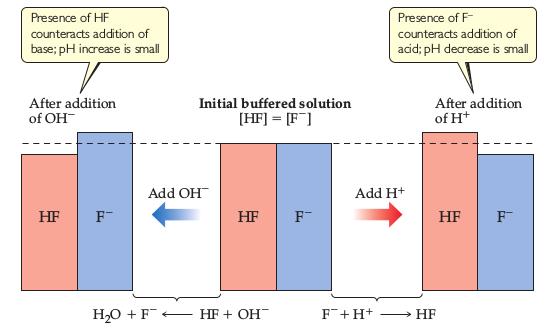
\includegraphics[width=\linewidth]{buffer_action.png}
\end{figure}
\end{multicols}
\end{mdframed}




\begin{mdframed}
\begin{multicols}{2}
\subsection{Acid-Base Titrations}
\begin{compactdesc}
    \item[pH titration curve] indicates pH as the titration progresses.
        See initial, equivalence and post-equivalnce values.
    \item[Equivalence point] moles of acid = moles of base
    \item[Strong base titrates strong acid] pH rises from about 0 to about
        14; equivalence point 7.
    \item[Strong acid titrates strong weak] pH lowers, same as base titrating
        acid.
    \item[Strong titrates weak] sudden change in pH, but equivalence point is
        closer. May not be 7 due to conjugate base/acid. Equivalence point pH increases
        as $k_a$ decreases, closer to titrator's side.
    \item[Acid-base indicator] can be used instead of pH meter. It must have
        an activation range near the equivalence point.
        Phenolphthalein range 8.3 to 10.0, Methyl red ranges from 4.2 to 6.0.
    \item[Polyprotic acids] curve with two equivalence points.
    \item[Half-equivalence point] $pH = pK_a$
\end{compactdesc}

\begin{figure}[H]
    \centering
    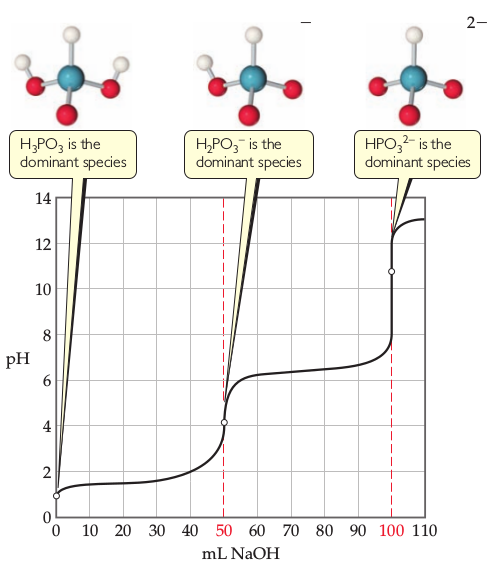
\includegraphics[width=0.8\linewidth]{polyprotic_titration.png}
\end{figure}
\end{multicols}
\end{mdframed}






\begin{mdframed}
\begin{multicols}{2}
\subsection{Solubility Equilibria}
\begin{compactdesc}
\item[Heterogeneous solubility] Species in different phases. Dissolution,
    precipitation of ionic compounds.
\item[Solubility-Product constant] $K_{sp}$ solubility of solid in water.
    $K_{sp} = $ product of concentrations of ions, raised to power of its
    equilibrium coefficient.
    \ce{CaF2} gives $K_{sp} = [\ce{Ca^{2+}}][\ce{F^-}]^2$. Small means
    it doesn't dissolve much.
\item[Solubility] is quantity that dissolves to form saturated soln,
    very volatile.
    $K_{sp}$ measures how much solid dissolves, one for each temperature
    (extreme accuracy? consider concentration).

\item[Solubility from $K_{sp}$] ICE table for dissolved ions, their initial conc.s are 0 unless otherwise noted. Only if no
    other important equilibria affecting solubility.
    Units: $\frac{g}{L \text{ soln}}$, $\frac{mol}{L     \text{ soln}}$.
\item[Deviations] caused by electrostatic between ions, ignoring
    acid-base equilibria, incomplete dissociation (like \ce{MgF+} ions)
\end{compactdesc}
\end{multicols}
\end{mdframed}




%TODO adding OH to soluble salt, ksp problem

\begin{mdframed}
\begin{multicols}{2}
\subsection{Factors affecting solubility}
\begin{compactdesc}
\item[Common-ion effect] generally, solubility of a slightly soluble salt
    decreased by common-ion. Shift left.
\item[pH affects solubility,] increases for basic anions.
    Can dissolve completely in very acidic solution.
    Example: \ce{Mg(OH)2 (s)} usually pH = 10.52 [\ce{Mg^{2+}}] = 0.00017, if
    pH is buffered to 9 and $K_{sp} = 1.8\cdot10^{-11}$ then [\ce{Mg^{2+}}]
    = 0.18M.
\item[Complex ion] very soluble in water. ...
\item[Formation of Complex ions]
\item[Formation constant]
\item[Amphoterism]
\end{compactdesc}
\end{multicols}
\end{mdframed}






\begin{mdframed}
\begin{multicols}{2}
\subsection{Precipitation and Separation of Ions}
\begin{compactdesc}
\item[Q for solubility] $K_{sp}$, but not necessarily at equilibrium.
Can use same as Q in Chapter 15 to find direction of the reaction.
\item[Q $= K_{sp}$] solution is saturated, no precipitate
\item[Q $< K_{sp}$] reaction proceeds to the right, no precipitate
\item[Q $> K_{sp}$] reaction proceeds to the left, precipitate
\item[Selective precipitation] ions can be separated based on solubilities of
    salts. Sulfide ion is commonly used, sulfide salts span wide range.
    CuS $K_{sp} = 6\cdot 10^{-37}$, ZnS $K_{sp} = 2\cdot 10^{-25}$.
    CuS will precipitate with pH around 1, ZnS will precipitate at higher
    pH.
\end{compactdesc}
\end{multicols}
\end{mdframed}






\begin{mdframed}
\begin{multicols}{2}
\subsection{Qualitivative Analysis for Metallic Elements}
\begin{compactdesc}
\item[Metals vary] in their salt solubility, acid-base, complex ions.
    These differences can be used to separate and detect presence of metal
    ions.
\item[Qualitative analysis] presence/absence of species
\item[Quantitative analysis] quantity of species
\item[Common 5 group scheme]
    \begin{compactdesc}
    \item[Group 1] insoluble chlorides, add \ce{HCl}, precipitates
        \ce{AgCl}, \ce{Hg2Cl2}, \ce{PbCl2}
    \item[Group 2] acid-insoluble sulfides, soln. now acidic, \ce{H2S} is
        added, precipitates \ce{CuS}, \ce{Bi2S3}, \ce{CdS}, \ce{PbS},
        \ce{HgS}, \ce{Ag2S3}, \ce{Sb2S3}, \ce{SnS2}. These have low
        $K_{sp}$
    \item[Group 3] base-insoluble sulfides and hydroxides, soln made basic,
        \ce{(NH4)2S} added, precipitates \ce{Al^{3+}}, \ce{Cr^{3+}},
        \ce{Fe^{3+}}, \ce{Zn^{2+}}, \ce{Ni^{2+}}, \ce{Co^{2+}},
        \ce{Mn^{2+}}
    \item[Group 4] insoluble phosphates, \ce{(NH4)2HPO4} precipitates
        \ce{Mg^{2+}}, \ce{Ca^{2+}}, \ce{Sr^{2+}}, \ce{Ba^{2+}}
    \item[Group 5] alkali metal, \ce{NH4+} flame test, other individual tests.
    \end{compactdesc}
\end{compactdesc}

\begin{figure}[H]
    \centering
    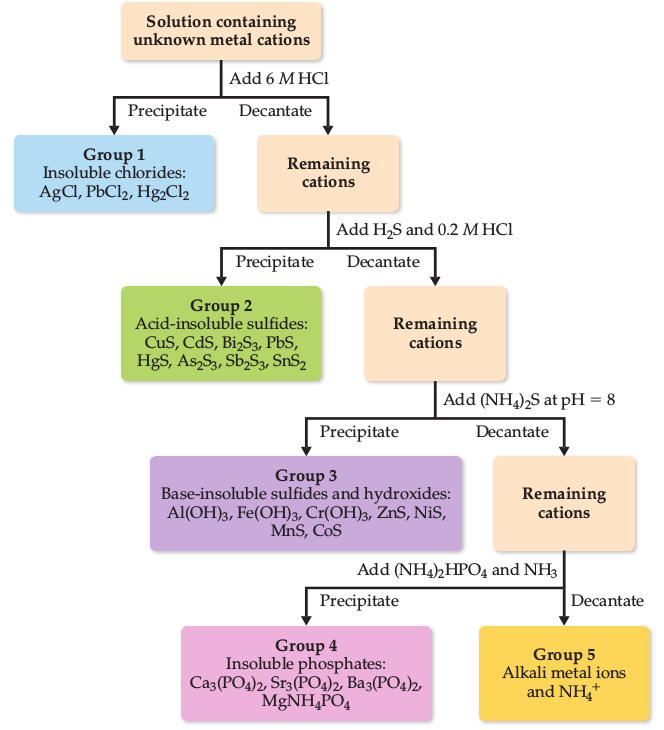
\includegraphics[width=0.9\linewidth]{cation_detection.png}
\end{figure}
\end{multicols}
\end{mdframed}






